\section{Incidence matrices}

Tangle diagrams essentially represent a combination of connections, i.e. strands connect crossings, like edges connect vertices on a graph. Given this similarity, we can construct incidence matrices for the crossings of our tangle diagrams. 

We construct an incidence matrix for a tangle diagram as follows:

\begin{enumerate}
\item Enumerate crossings in order of occurence in the tangle, if we have encountered a crossing before, we skip it. Prepare an ``empty" square matrix $A\in M(n,\{R,G,B,W\})$ where $n$ is the number of crossings, and $R,G,B,W$ represent red, green, blue, and white.
\item For each crossing $i$ in the order, making note of the orientation, we fill entries of $A$ with
\begin{itemize}
\item $A_{ji}=R$
\item $A_{ii}=G$
\item $A_{ki}=B$
\item for all $m\not\in\{i,j,k\}$, $A_{mi}=W$, 
\end{itemize}
where $j,k$ are the crossings left of and right of the crossing $i$ with respect to the over strand, refer to \Cref{fig:incidence} for details
\end{enumerate}

\begin{figure}[h!]
\centering
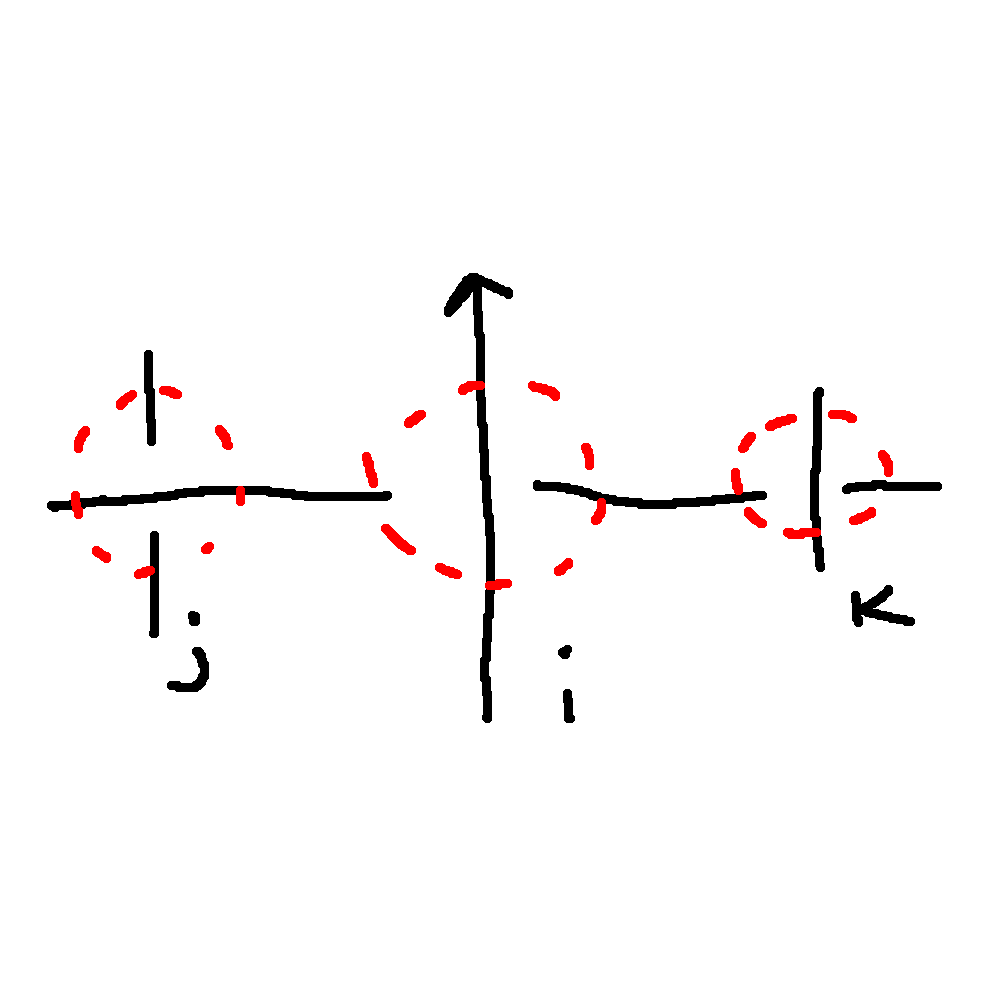
\includegraphics[width=0.4\textwidth]{incidence.png}
\caption{Following the orientation of the crossing $i$, with respect to the over strand, the left crossing is $j$ and the right crossing is $k$. The orientation of the crossings $j,k$ is not important.}
\label{fig:incidence}
\end{figure}

So in other words, each column represents a crossing, and we only consider what is on either side of the crossing. Reading the columns from left to right we get a sense of what crossings are hit. We picked $R,G,B,W$ symbolically, since we wish to plot the matrices, and after a few iterations, any numerical symbols will be illegible. 

We plot some incidence matrices of tangles diagrams corresponding to closed knots from the Rolfsen knot table as found in \citep{rolfsen}. We see interesting patterns emerge! In \Cref{fig:trefR1examples} we have a few instances of the trefoil tangle diagram with an R1 loop added between some crossings, we see that there is some variation after a number of iterations. This variation does not seem to be consistent since the two lower examples have nearly the same incidence matrices, however the first example differs greatly, e.g. the side bands are closer to the diagonal, and the pattern around the diagonal is different.

In \Cref{fig:varioustangleexamples} we have a few more examples but of different tangles. We see similar kind of behavior that as before, some have similar structures, for example, the trefoil and 4,1 have about the same arrangement of squares, the bands and off diagonal patterns, except the colors change. However if we compare them with 9,10 and 10,23, we see variation in features between those two examples, and the previous trefoil and 4,1.

We see distinct and recognisable structures, yet it is not clear what the mechanism behind their production could be.

\newpage

\begin{figure}[H]
\centering
\begin{subfigure}[t]{0.48\textwidth}
\centering
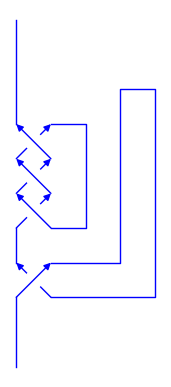
\includegraphics[width=0.30\textwidth]{3_1_ed_0.png}
\end{subfigure}
\hfill
\begin{subfigure}[t]{0.48\textwidth}
\centering
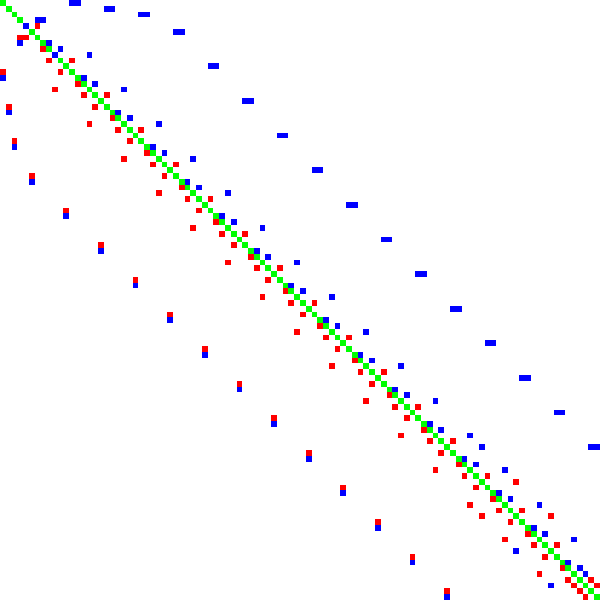
\includegraphics[width=0.8\textwidth]{3_1_R1at0_50.png}
\end{subfigure}
\hfill
\begin{subfigure}[t]{0.48\textwidth}
\centering
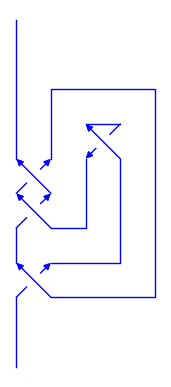
\includegraphics[width=0.3\textwidth]{3_1_ed_2.png}
\end{subfigure}
\hfill
\begin{subfigure}[t]{0.48\textwidth}
\centering
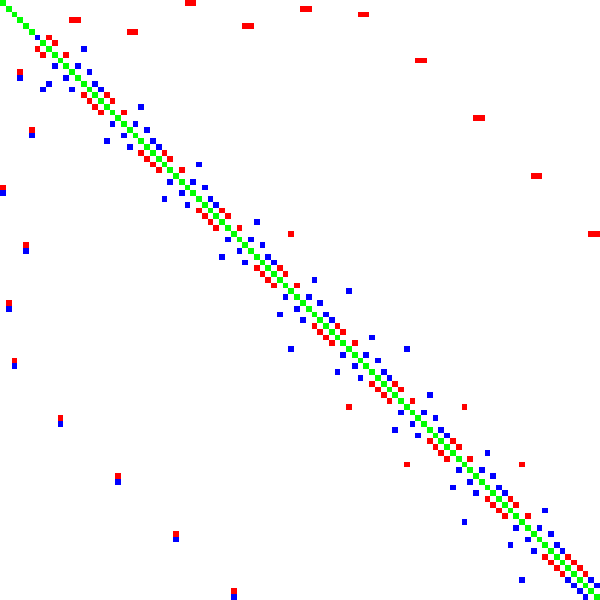
\includegraphics[width=0.8\textwidth]{3_1_R1at2_50.png}
\end{subfigure}
\hfill
\begin{subfigure}[t]{0.48\textwidth}
\centering
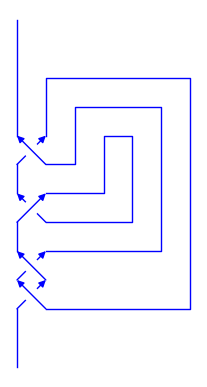
\includegraphics[width=0.3\textwidth]{3_1_ed_4.png}
\end{subfigure}
\hfill
\begin{subfigure}[t]{0.48\textwidth}
\centering
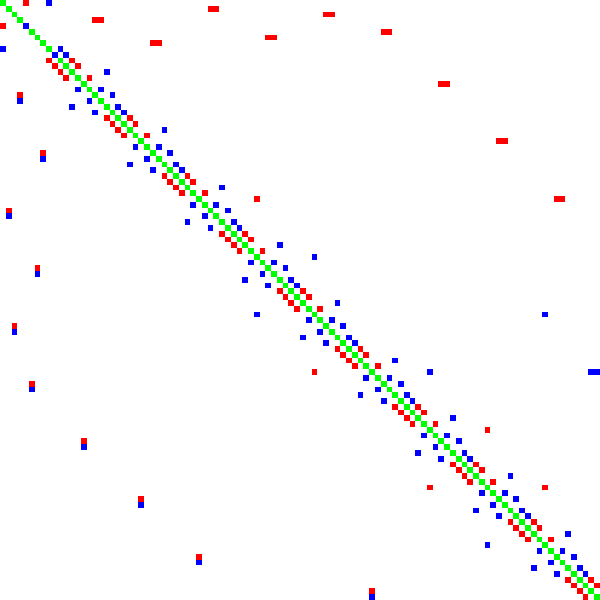
\includegraphics[width=0.8\textwidth]{3_1_R1at4_50.png}
\end{subfigure}
\caption{On the left are diagrams of the trefoil with added R1 loops, on the right their respective incidence matrices after 50 iterations of the OU algorithm}
\label{fig:trefR1examples}
\end{figure}

\begin{figure}[H]
\centering
\begin{subfigure}{0.24\textwidth}
\centering
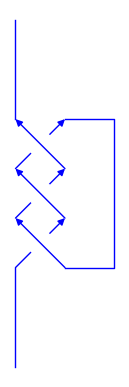
\includegraphics[height=0.25\textheight]{my_trefoil.png} \vfill
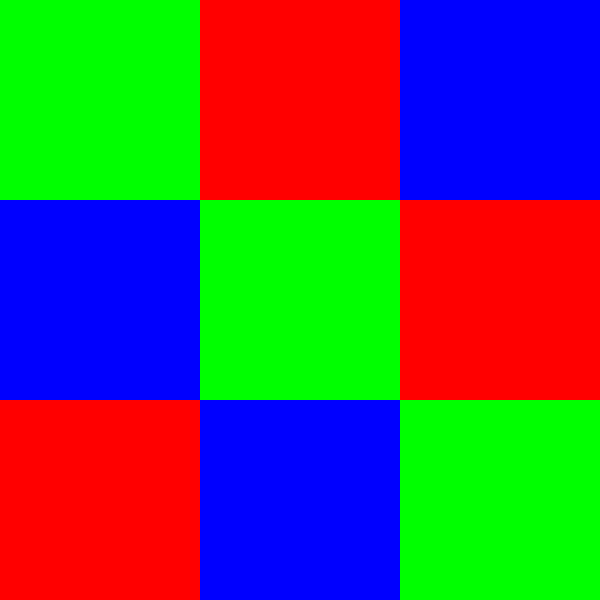
\includegraphics[height=0.15\textheight]{3_1_0.png}       \vfill\vspace{1mm}
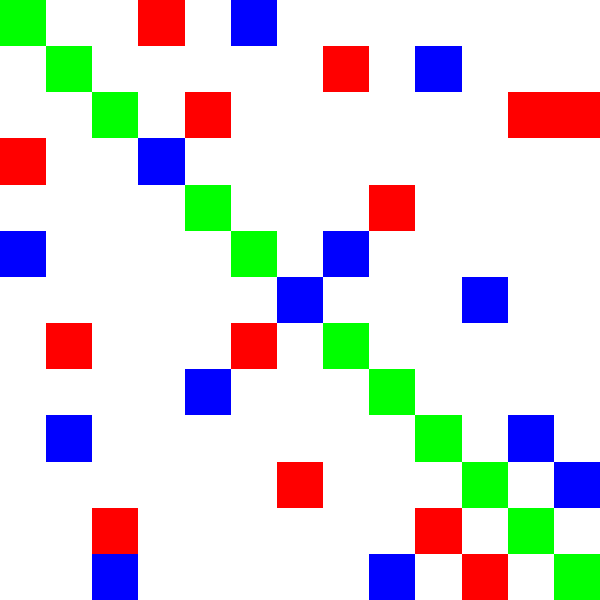
\includegraphics[height=0.15\textheight]{3_1_5.png}       \vfill\vspace{1mm}
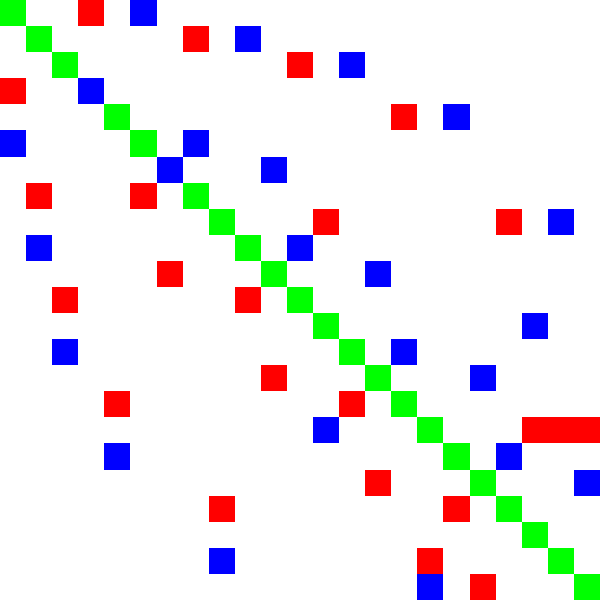
\includegraphics[height=0.15\textheight]{3_1_10.png}      \vfill\vspace{1mm}
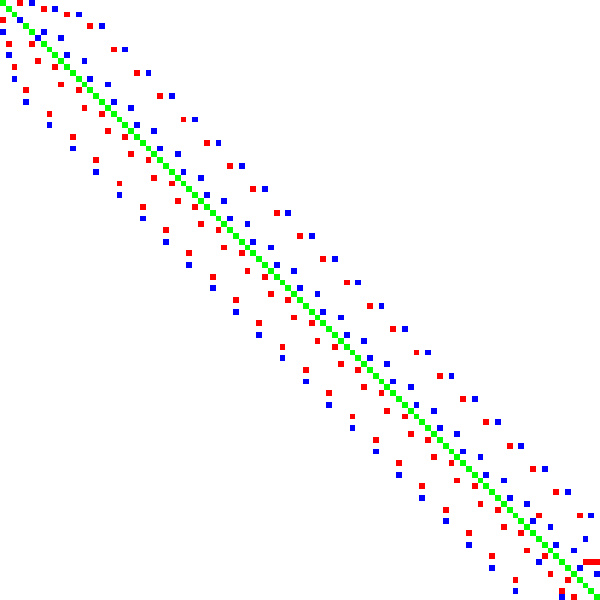
\includegraphics[height=0.15\textheight]{3_1_50.png}
\caption{trefoil diagram}
\end{subfigure}
\hfill
\begin{subfigure}{0.24\textwidth}
\centering
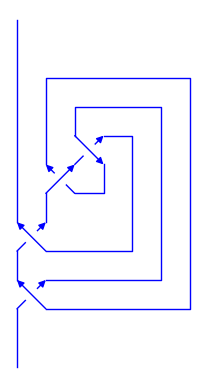
\includegraphics[height=0.25\textheight]{my_4_1.png} \vfill
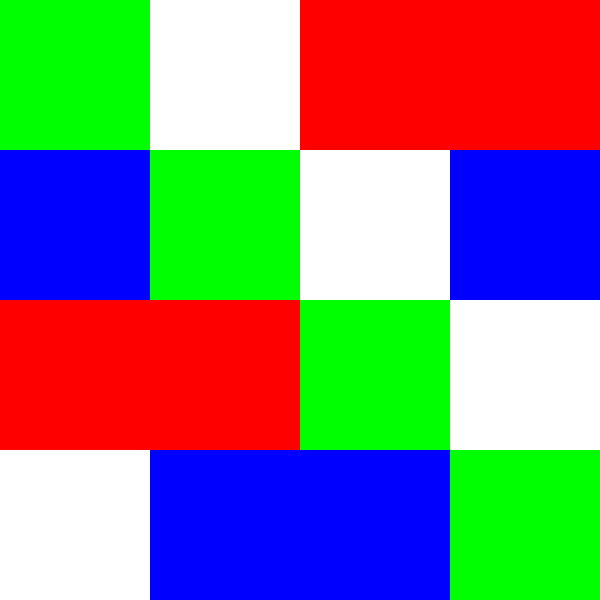
\includegraphics[height=0.15\textheight]{4_1_0.png}  \vfill\vspace{1mm}
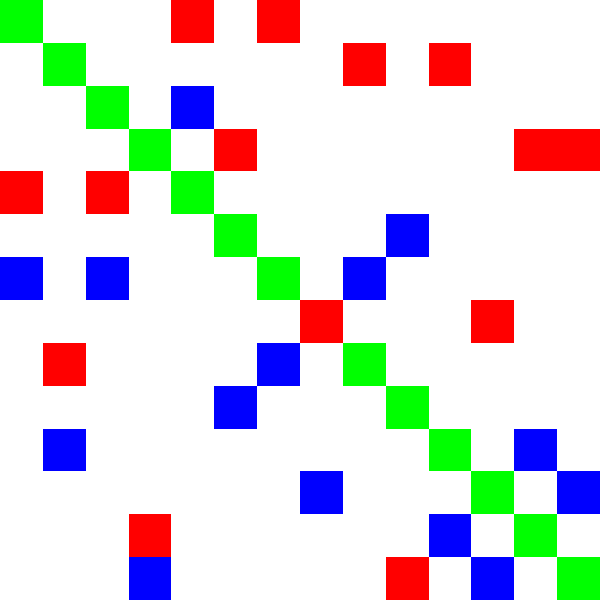
\includegraphics[height=0.15\textheight]{4_1_5.png}  \vfill\vspace{1mm}
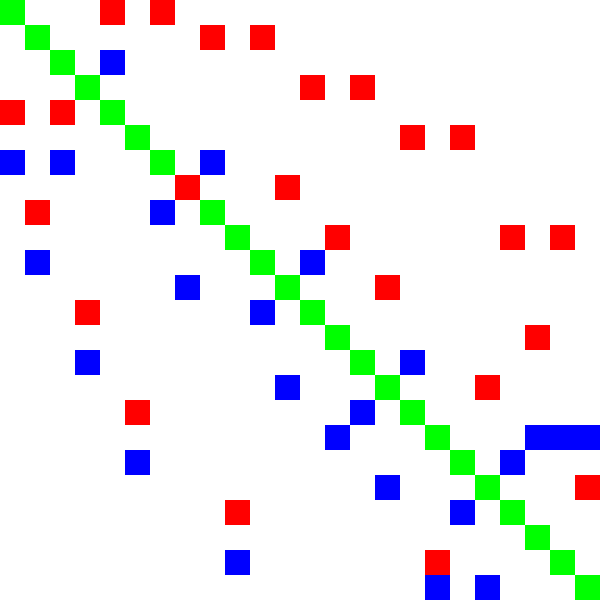
\includegraphics[height=0.15\textheight]{4_1_10.png} \vfill\vspace{1mm}
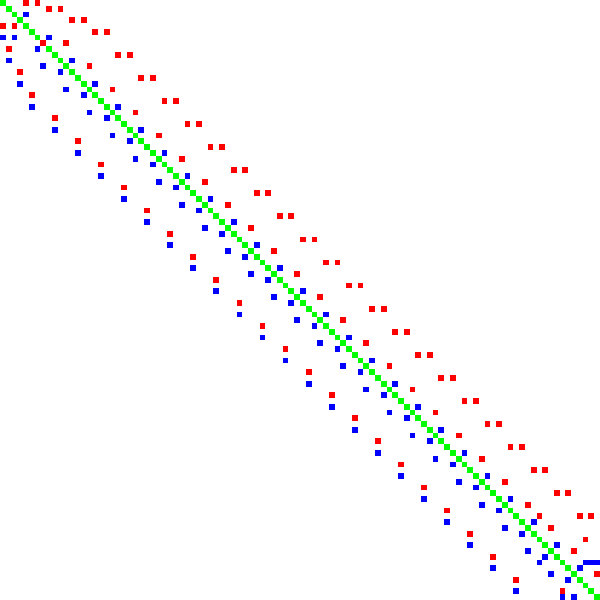
\includegraphics[height=0.15\textheight]{4_1_50.png} \vfill\vspace{1mm}
\caption{4,1 diagram}
\end{subfigure}
\hfill
\begin{subfigure}{0.24\textwidth}
\centering
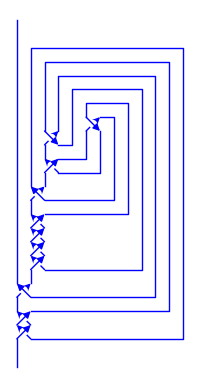
\includegraphics[height=0.25\textheight]{my_9_10.png} \vfill
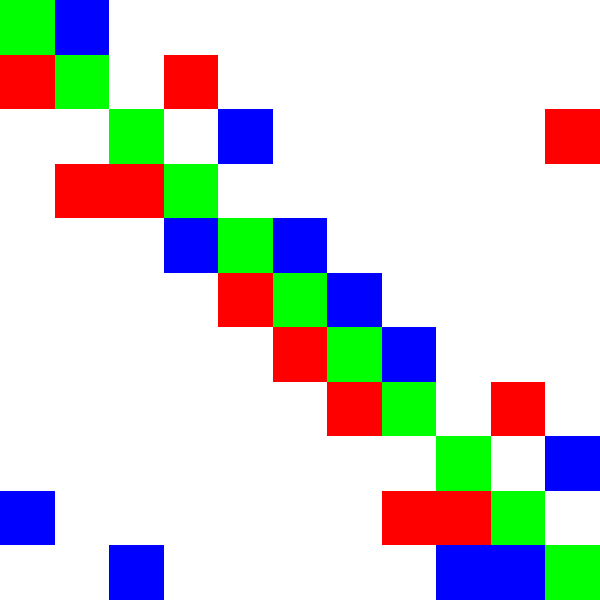
\includegraphics[height=0.15\textheight]{9_10_0.png}  \vfill\vspace{1mm}
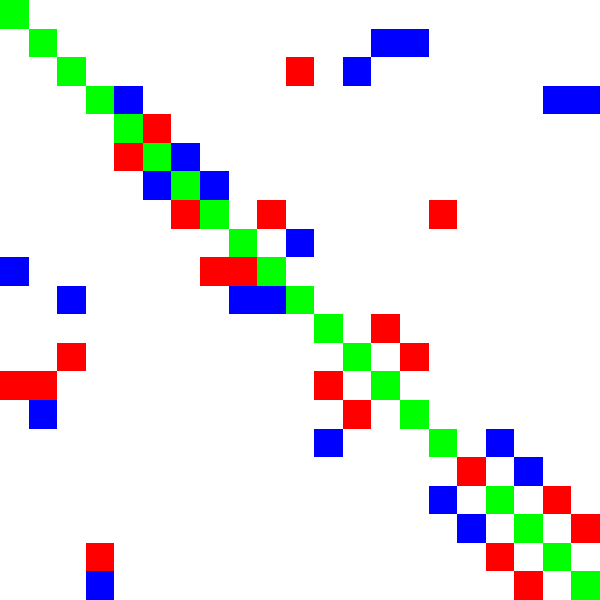
\includegraphics[height=0.15\textheight]{9_10_5.png}  \vfill\vspace{1mm}
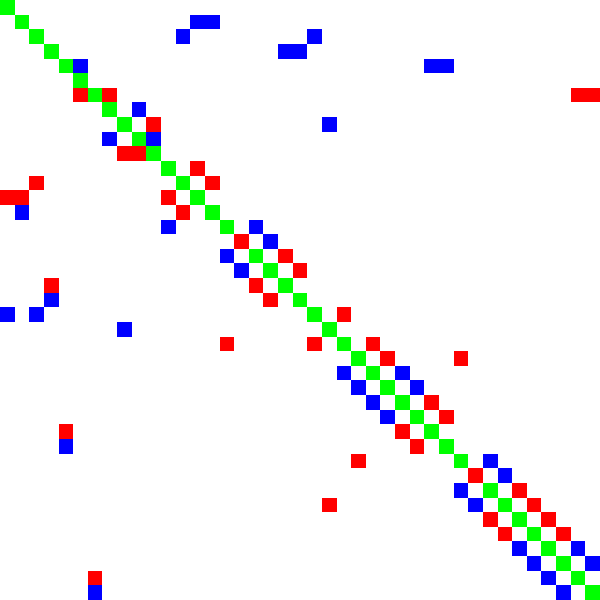
\includegraphics[height=0.15\textheight]{9_10_10.png} \vfill\vspace{1mm}
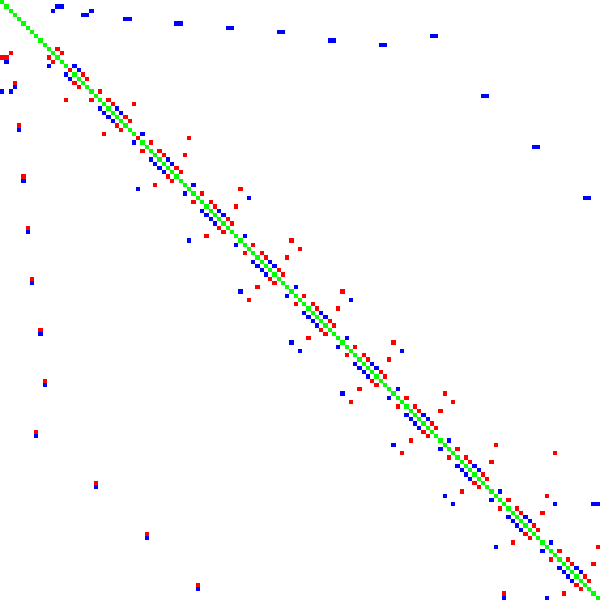
\includegraphics[height=0.15\textheight]{9_10_50.png} \vfill\vspace{1mm}
\caption{9,10 diagram}
\end{subfigure}
\hfill
\begin{subfigure}{0.24\textwidth}
\centering
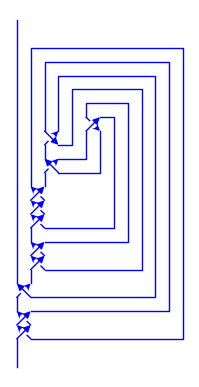
\includegraphics[height=0.25\textheight]{my_10_50.png} \vfill
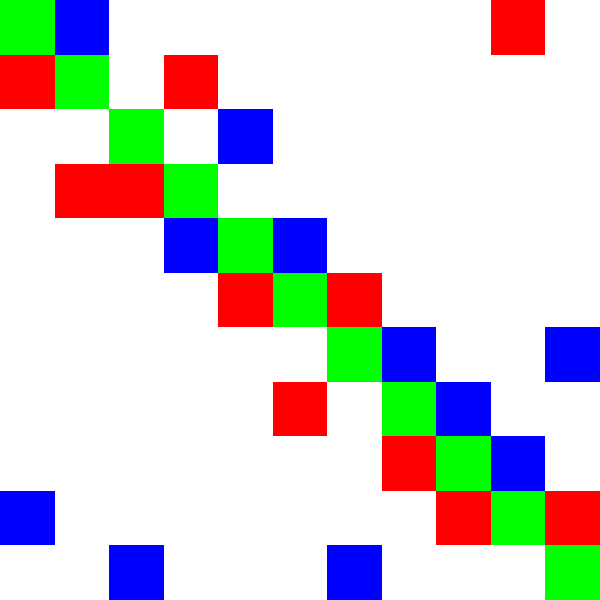
\includegraphics[height=0.15\textheight]{10_50_0.png}  \vfill\vspace{1mm}
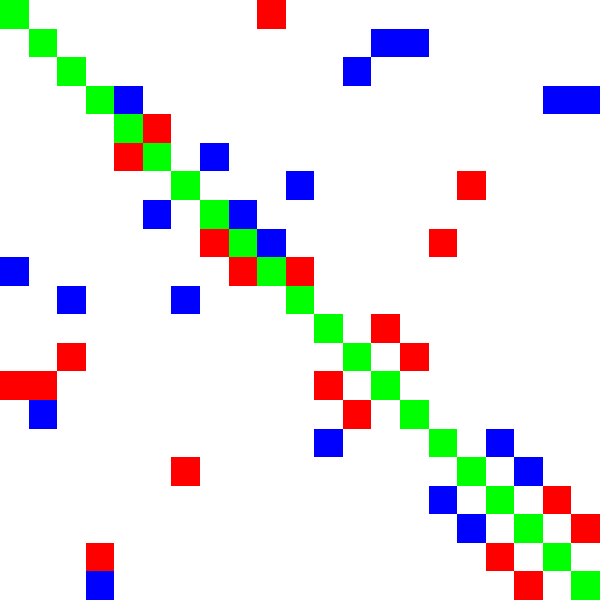
\includegraphics[height=0.15\textheight]{10_50_5.png}  \vfill\vspace{1mm}
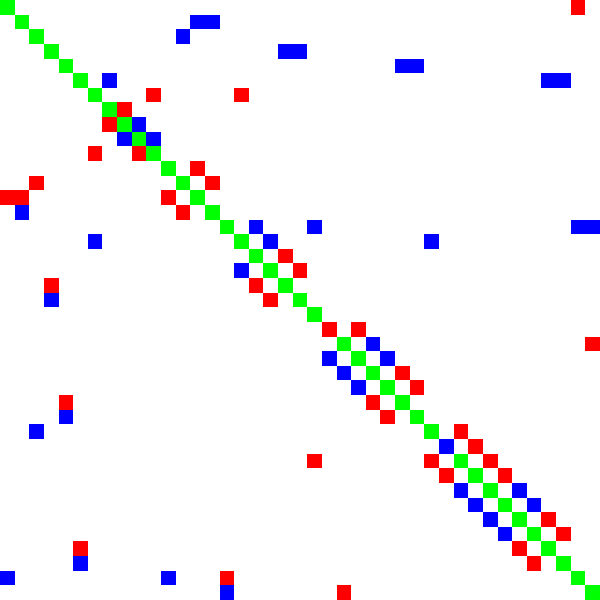
\includegraphics[height=0.15\textheight]{10_50_10.png} \vfill\vspace{1mm}
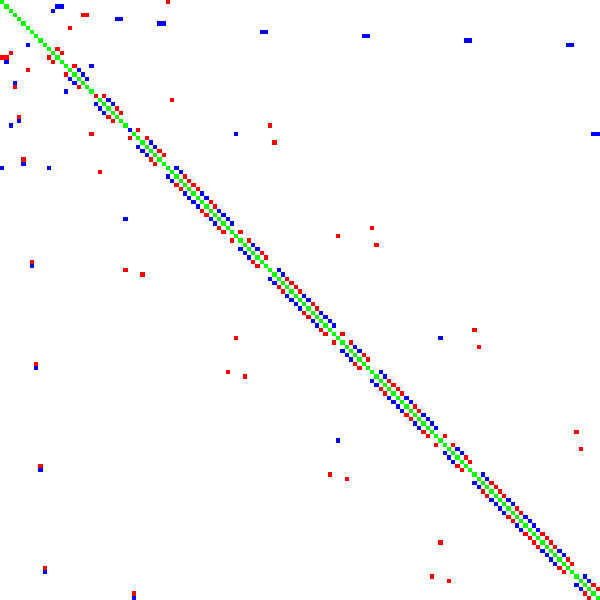
\includegraphics[height=0.15\textheight]{10_50_50.png} \vfill\vspace{1mm}
\caption{10,23 diagram}
\end{subfigure}
\caption{Comparing incidence matrices of several tangles diagrams under the OU algorithm. Each column is a separate tangle, each column is 0, 5, 10, 50 iterations}
\label{fig:varioustangleexamples}
\end{figure}